\documentclass[a4paper]{article}
\usepackage[a4paper,margin=0mm]{geometry}
\usepackage{fontspec}
\usepackage{unicode-math}
\usepackage{tikz}
\usepackage[table]{xcolor}
\usepackage[absolute]{textpos}
\usepackage{enumitem}
\usepackage{array}
\usepackage{multirow}

\setmainfont{Libertinus Serif}
\setsansfont{Libertinus Sans}
\setmathfont{Libertinus Math}
\newfontfamily\trackedsans{Libertinus Sans}[LetterSpace=8.0]

\definecolor{accent}{HTML}{F46530}
\definecolor{badge}{HTML}{FFBDA5}
\definecolor{ink}{HTML}{2A2E30}

\setlength{\TPHorizModule}{1mm}
\setlength{\TPVertModule}{1mm}
\setlength{\parindent}{0pt}
\pagestyle{empty}

% ---- Safe print margins: 16mm outer on both sides so bound/trimmed copies never
% clip problem text. Columns are 83mm wide with a 6mm gap on each side of the
% center rule (at x=105mm). ----
\newcommand{\LCOL}{16mm}
\newcommand{\RCOL}{111mm}
\newcommand{\COLW}{83mm}

% ---- Plain topic header: number chip + title, thin rule underneath. No band, no watermark. ----
\newcommand{\topicheader}[2]{%
\begin{textblock*}{194mm}(16mm,10mm)
\begin{tikzpicture}
\node[fill=accent,text=white,font=\sffamily\bfseries\fontsize{13}{13}\selectfont,
      minimum width=9mm,minimum height=9mm,inner sep=0pt] at (4.5mm,-4.5mm) {#1};
\node[font=\sffamily\bfseries\fontsize{15}{16}\selectfont,text=ink,anchor=west] at (12mm,-4.5mm) {#2};
\end{tikzpicture}
\end{textblock*}
\begin{textblock*}{194mm}(16mm,22.5mm)

\begin{tikzpicture}
\fill[accent] (0,0) rectangle (194mm,0.5mm);
\end{tikzpicture}
\end{textblock*}
}

\newcommand{\pagefooter}[1]{%
\begin{textblock*}{194mm}(8mm,286.41mm)
  
\begin{tikzpicture}
    \fill[accent] (0,0) rectangle (194mm,0.6mm);
  \end{tikzpicture}
\end{textblock*}
\begin{textblock*}{63.59mm}(8mm,288.27mm)
  {\sffamily\bfseries\color{accent}\fontsize{13}{16}\selectfont SAT 1200+}
\end{textblock*}
\begin{textblock*}{10mm}(188mm,288.27mm)
  \centering{\sffamily\color{accent}\fontsize{14}{16}\selectfont #1}
\end{textblock*}
}

% ---- Fixed-length vertical column rule: #1 = top y (mm), #2 = length (mm) ----
\newcommand{\colrule}[2]{%
\begin{textblock*}{1mm}(105mm,#1mm)
\begin{tikzpicture}
\draw[black!65,line width=0.5pt] (0,0) -- (0,#2mm);
\end{tikzpicture}
\end{textblock*}
}

\newcommand{\setkicker}[2]{%
{\sffamily\bfseries\fontsize{12}{14}\selectfont #1.}\ {\itshape\fontsize{11}{14}\selectfont\color{black!75} #2}\par\vspace{2mm}%
}

% ---- Small boxed problem number, reference-style. Plain \fbox -- stays flush with
% the text baseline instead of centering on it. ----
\setlength{\fboxsep}{1.4pt}
\setlength{\fboxrule}{0.5pt}
\newcommand{\pnum}[1]{\fcolorbox{ink}{white}{\sffamily\bfseries\fontsize{8}{8}\selectfont #1}~}

% ---- QR placeholder square + caption below ----
\newcommand{\qrbox}[1]{%
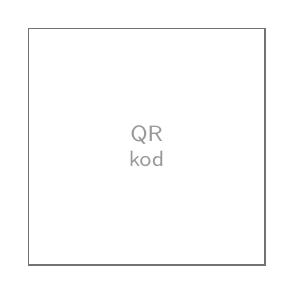
\begin{tikzpicture}
\draw[black!55,line width=0.6pt] (0,0) rectangle (30mm,30mm);
\node[black!40,font=\sffamily\fontsize{8}{9}\selectfont,align=center] at (15mm,15mm) {QR\\kod};
\end{tikzpicture}\\[1.5mm]
{\sffamily\fontsize{9}{11}\selectfont\color{black!70} #1}%
}

% ---- Answer-table styling: accent-colored grid, like the reference "Number | Answer" table ----
\arrayrulecolor{accent}
\setlength{\arrayrulewidth}{0.7pt}
\renewcommand{\arraystretch}{1.35}
\newcommand{\anstitle}[1]{{\sffamily\bfseries\color{accent}\fontsize{11}{13}\selectfont #1}\\[1.3mm]}

\begin{document}

% ================= PAGE 1: Set 1 | Set 2 =================
\topicheader{6}{Kvadrat Tenglamalar: To'liq Kvadrat va Formula}
\pagefooter{1}
\colrule{32}{238}
\mbox{}%

\begin{textblock*}{\COLW}(\LCOL,32mm)
{\fontsize{12}{15}\selectfont
\setkicker{1-to'plam}{Har birini $a(x-h)^2+k$ ko'rinishiga keltiring (to'liq kvadratga keltirish).}

\noindent\pnum{1} $y=x^2-4x+3$\\[26mm]
\noindent\pnum{2} $y=x^2+2x-5$\\[26mm]
\noindent\pnum{3} $y=x^2-8x+10$\\[26mm]
\noindent\pnum{4} $y=x^2+6x+4$\\[26mm]
\noindent\pnum{5} $y=x^2-10x+21$\\[26mm]
\noindent\pnum{6} $y=x^2+2x+1$
}
\end{textblock*}

\begin{textblock*}{\COLW}(\RCOL,32mm)
{\fontsize{12}{15}\selectfont
\setkicker{2-to'plam}{Kvadrat tenglama formulasi bilan yeching (diskriminant aniq kvadrat).}

\noindent\pnum{1} $x^2-5x+6=0$\\[30mm]
\noindent\pnum{2} $x^2+x-6=0$\\[30mm]
\noindent\pnum{3} $2x^2-3x-2=0$\\[30mm]
\noindent\pnum{4} $x^2-9=0$\\[30mm]
\noindent\pnum{5} $3x^2+5x+2=0$\\[30mm]
\noindent\pnum{6} $x^2-7x+12=0$
}
\end{textblock*}

\clearpage

% ================= PAGE 2: Set 3 | Set 4 =================
\topicheader{6}{Kvadrat Tenglamalar: To'liq Kvadrat va Formula}
\pagefooter{2}
\colrule{32}{238}
\mbox{}%

\begin{textblock*}{\COLW}(\LCOL,32mm)
{\fontsize{12}{15}\selectfont
\setkicker{3-to'plam}{Formula bilan yeching -- ildizlar irratsional bo'ladi.}

\noindent\pnum{1} $x^2-4x+1=0$\\[30mm]
\noindent\pnum{2} $x^2+2x-4=0$\\[30mm]
\noindent\pnum{3} $2x^2-4x-1=0$\\[30mm]
\noindent\pnum{4} $x^2-6x+7=0$\\[30mm]
\noindent\pnum{5} $x^2+4x+2=0$\\[30mm]
\noindent\pnum{6} $3x^2-6x+2=0$
}
\end{textblock*}

\begin{textblock*}{\COLW}(\RCOL,32mm)
{\fontsize{12}{15}\selectfont
\setkicker{4-to'plam}{Aralash -- to'liq kvadratga keltirish yoki formula, o'zingiz tanlang.}

\noindent\pnum{1} $x^2+8x+15=0$\\[40mm]
\noindent\pnum{2} $x^2-2x-5=0$\\[40mm]
\noindent\pnum{3} $4x^2-4x-3=0$\\[40mm]
\noindent\pnum{4} $x^2+5x+3=0$
}
\end{textblock*}

\clearpage

% ================= PAGE 3: Set 5 (verify both roots) | Set 6 (spot the error) =================
\topicheader{6}{Kvadrat Tenglamalar: To'liq Kvadrat va Formula}
\pagefooter{3}
\colrule{32}{238}
\mbox{}%

\begin{textblock*}{\COLW}(\LCOL,32mm)
{\fontsize{12}{15}\selectfont
\setkicker{5-to'plam}{Ikkala ildizni toping, so'ng har birini asl tenglamaga qo'yib tekshiring.}

\noindent\pnum{1} $x^2-x-12=0$\\[50mm]
\noindent\pnum{2} $x^2+3x-10=0$\\[50mm]
\noindent\pnum{3} $2x^2+x-6=0$
}
\end{textblock*}

\begin{textblock*}{\COLW}(\RCOL,32mm)
{\fontsize{11}{14}\selectfont
\setkicker{6-to'plam}{Xatoni toping -- buzilgan qadamni ayting, to'g'ri javobni bering.}

\noindent\pnum{1} $x^2-6x+4=0$ ifodasida ko'rsatilgan yechimda xato bor:\\[1mm]
\hspace*{7mm}\textit{``$x=\dfrac{-6\pm\sqrt{36-16}}{2}$''}\\[2mm]
\hspace*{7mm}Xato va to'g'ri javob: \makebox[52mm]{\dotfill}\\[16mm]

\noindent\pnum{2} $x^2+2x-2=0$ ifodasida ko'rsatilgan yechimda xato bor:\\[1mm]
\hspace*{7mm}\textit{``Diskriminant $=4-8=-4$, $x=\dfrac{-2\pm\sqrt{-4}}{2}$''}\\[2mm]
\hspace*{7mm}Xato va to'g'ri javob: \makebox[52mm]{\dotfill}\\[16mm]

\noindent\pnum{3} $x^2-4x-1=0$ ifodasida ko'rsatilgan yechimda xato bor:\\[1mm]
\hspace*{7mm}\textit{``$x=\dfrac{4+\sqrt{20}}{2}=2+\sqrt5$. Javob: $x=2+\sqrt5$.''}\\[2mm]
\hspace*{7mm}Xato va to'g'ri javob: \makebox[52mm]{\dotfill}
}
\end{textblock*}

\clearpage

% ================= PAGE 4: Set 7 (bonus, a != 1) -- own page; answers follow on a fresh page =================
\topicheader{6}{Kvadrat Tenglamalar: To'liq Kvadrat va Formula}
\pagefooter{4}
\colrule{32}{238}
\mbox{}%

\begin{textblock*}{\COLW}(\LCOL,32mm)
{\fontsize{12}{15}\selectfont
\setkicker{7-to'plam}{Bonus / qiyin -- $a\ne1$ bo'lgan hollar.}

\noindent\pnum{1} $2x^2+6x+3=0$\\[45mm]
\noindent\pnum{2} $3x^2-2x-2=0$\\[45mm]
\noindent\pnum{3} $5x^2+4x-1=0$\\[45mm]
\noindent\pnum{4} $2x^2-7x+4=0$
}
\end{textblock*}

\clearpage

% ================= PAGE 5: Javoblar -- full-page answer table, own page always =================
\topicheader{6}{Kvadrat Tenglamalar: To'liq Kvadrat va Formula}
\pagefooter{5}
\mbox{}%

\begin{textblock*}{194mm}(16mm,30mm)
{\bfseries\itshape\color{accent}\fontsize{19}{21}\selectfont\centering Javoblar\par}
\end{textblock*}

\begin{textblock*}{194mm}(16mm,44mm)
{\fontsize{9.5}{12}\selectfont
\centering
\renewcommand{\arraystretch}{1.35}
\begin{tabular}{|>{\centering\arraybackslash}p{24mm}|>{\centering\arraybackslash}p{9mm}|>{\centering\arraybackslash}p{34mm}|>{\centering\arraybackslash}p{9mm}|>{\centering\arraybackslash}p{34mm}|}
\hline
\rowcolor{badge!55}\textbf{To'plam} & \textbf{\#} & \textbf{Javob} & \textbf{\#} & \textbf{Javob}\\
\hline
\multirow{3}{24mm}{\centering 1-to'plam} & 1 & $(x-2)^2-1$ & 2 & $(x+1)^2-6$\\\cline{2-5}
 & 3 & $(x-4)^2-6$ & 4 & $(x+3)^2-5$\\\cline{2-5}
 & 5 & $(x-5)^2-4$ & 6 & $(x+1)^2$\\\hline
\multirow{3}{24mm}{\centering 2-to'plam} & 1 & $x=2,3$ & 2 & $x=-3,2$\\\cline{2-5}
 & 3 & $x=-\frac12,2$ & 4 & $x=\pm3$\\\cline{2-5}
 & 5 & $x=-1,-\frac23$ & 6 & $x=3,4$\\\hline
\multirow{3}{24mm}{\centering 3-to'plam} & 1 & $x=2\pm\sqrt3$ & 2 & $x=-1\pm\sqrt5$\\\cline{2-5}
 & 3 & $x=1\pm\frac{\sqrt6}{2}$ & 4 & $x=3\pm\sqrt2$\\\cline{2-5}
 & 5 & $x=-2\pm\sqrt2$ & 6 & $x=1\pm\frac{\sqrt3}{3}$\\\hline
\multirow{2}{24mm}{\centering 4-to'plam} & 1 & $x=-5,-3$ & 2 & $x=1\pm\sqrt6$\\\cline{2-5}
 & 3 & $x=-\frac12,\frac32$ & 4 & $x=\frac{-5\pm\sqrt{13}}{2}$\\\hline
\multirow{2}{24mm}{\centering 5-to'plam} & 1 & $x=-3,4$ & 2 & $x=-5,2$\\\cline{2-5}
 & 3 & $x=-2,\frac32$ & -- & (barchasi $0$ga tekshiriladi)\\\hline
\multirow{2}{24mm}{\centering 7-to'plam} & 1 & $x=-\frac32\pm\frac{\sqrt3}{2}$ & 2 & $x=\frac13\pm\frac{\sqrt7}{3}$\\\cline{2-5}
 & 3 & $x=-1,\frac15$ & 4 & $x=\frac74\pm\frac{\sqrt{17}}{4}$\\\hline
\multirow{3}{24mm}{\centering 6-to'plam} & \multicolumn{4}{p{86mm}|}{1.\ Xato -- $-b=6$ o'rniga $b=-6$ ishlatilgan. To'g'ri: $x=3\pm\sqrt5$.}\\\cline{2-5}
 & \multicolumn{4}{p{86mm}|}{2.\ Xato -- diskriminant hisobi: $b^2-4ac=4-4(1)(-2)=4+8=12$, $-4$ emas. To'g'ri: $x=-1\pm\sqrt3$.}\\\cline{2-5}
 & \multicolumn{4}{p{86mm}|}{3.\ Xato -- faqat bitta ildiz bilan to'xtagan. To'g'ri: $x=2\pm\sqrt5$ (ikkalasi ham).}\\\hline
\end{tabular}
}
\end{textblock*}

\begin{textblock*}{194mm}(16mm,230mm)
\centering
{\sffamily\fontsize{9.5}{11.5}\selectfont\color{black!70} Video yechimlar va qo'shimcha testlar uchun quyidagi QR kodlarni skanerlang:}\\[4mm]
\begin{minipage}[t]{32mm}\centering\qrbox{YouTube}\end{minipage}%
\hspace{16mm}%
\begin{minipage}[t]{32mm}\centering\qrbox{Telegram}\end{minipage}
\end{textblock*}

\end{document}
